% ============================================================================
%  ESP32-Based Flame Detection System - Project Report
%  ----------------------------------------------------------------------------
%  Build: pdflatex (UTF-8). Recommended: Overleaf or local TeX Live / MiKTeX.
%    pdflatex rapor.tex   (run twice for the table of contents)
%  Images: in report/images/ (ASCII names).
% ============================================================================
\documentclass[11pt,a4paper]{article}

% Engine-dependent font setup: pdfLaTeX -> inputenc/fontenc; XeLaTeX/LuaLaTeX -> fontspec
\usepackage{iftex}
\ifPDFTeX
  \usepackage[utf8]{inputenc}
  \usepackage[T1]{fontenc}
  \usepackage{lmodern}
\else
  \usepackage{fontspec}
\fi
% shorthands=off: keeps babel shorthand characters from clashing with graphicx
\usepackage[english,shorthands=off]{babel}

\usepackage[a4paper,margin=2.5cm]{geometry}
\usepackage{graphicx}
\graphicspath{{images/}}
\usepackage{booktabs}
\usepackage{array}
\usepackage{xcolor}
\usepackage{float}
\usepackage{enumitem}
\usepackage{caption}
\usepackage{fancyhdr}
\usepackage{tikz}
\usetikzlibrary{positioning, arrows.meta}

\usepackage[hidelinks,unicode=true]{hyperref}
\hypersetup{
  pdftitle={ESP32-Based Flame Detection System - Project Report},
  pdfauthor={Yasin},
  colorlinks=true,
  linkcolor=black,
  urlcolor=blue!60!black,
  citecolor=black
}

% --- Color palette ---
\definecolor{flamered}{HTML}{C0392B}
\definecolor{flameorange}{HTML}{E67E22}
\definecolor{deepblue}{HTML}{1F3A5F}
\definecolor{lightgray}{HTML}{F2F4F7}
\definecolor{codebg}{HTML}{F6F8FA}

% --- Header / footer ---
\pagestyle{fancy}
\fancyhf{}
\lhead{\small Flame Detection System}
\rhead{\small Project Report}
\cfoot{\thepage}
\renewcommand{\headrulewidth}{0.4pt}

% --- Table column types ---
\newcolumntype{L}[1]{>{\raggedright\arraybackslash}p{#1}}
\captionsetup{font=small, labelfont=bf}

\usepackage{fancyvrb}

\begin{document}

% ============================================================================
%  COVER
% ============================================================================
\begin{titlepage}
\centering
\vspace*{1.0cm}

{\Huge\bfseries ESP32-Based Flame Detection\\[0.3cm] and Real-Time Monitoring System\par}
\vspace{0.5cm}

{\Large An Internet of Things (IoT) Based\\ Early Fire Warning Project\par}
\vspace{1.1cm}

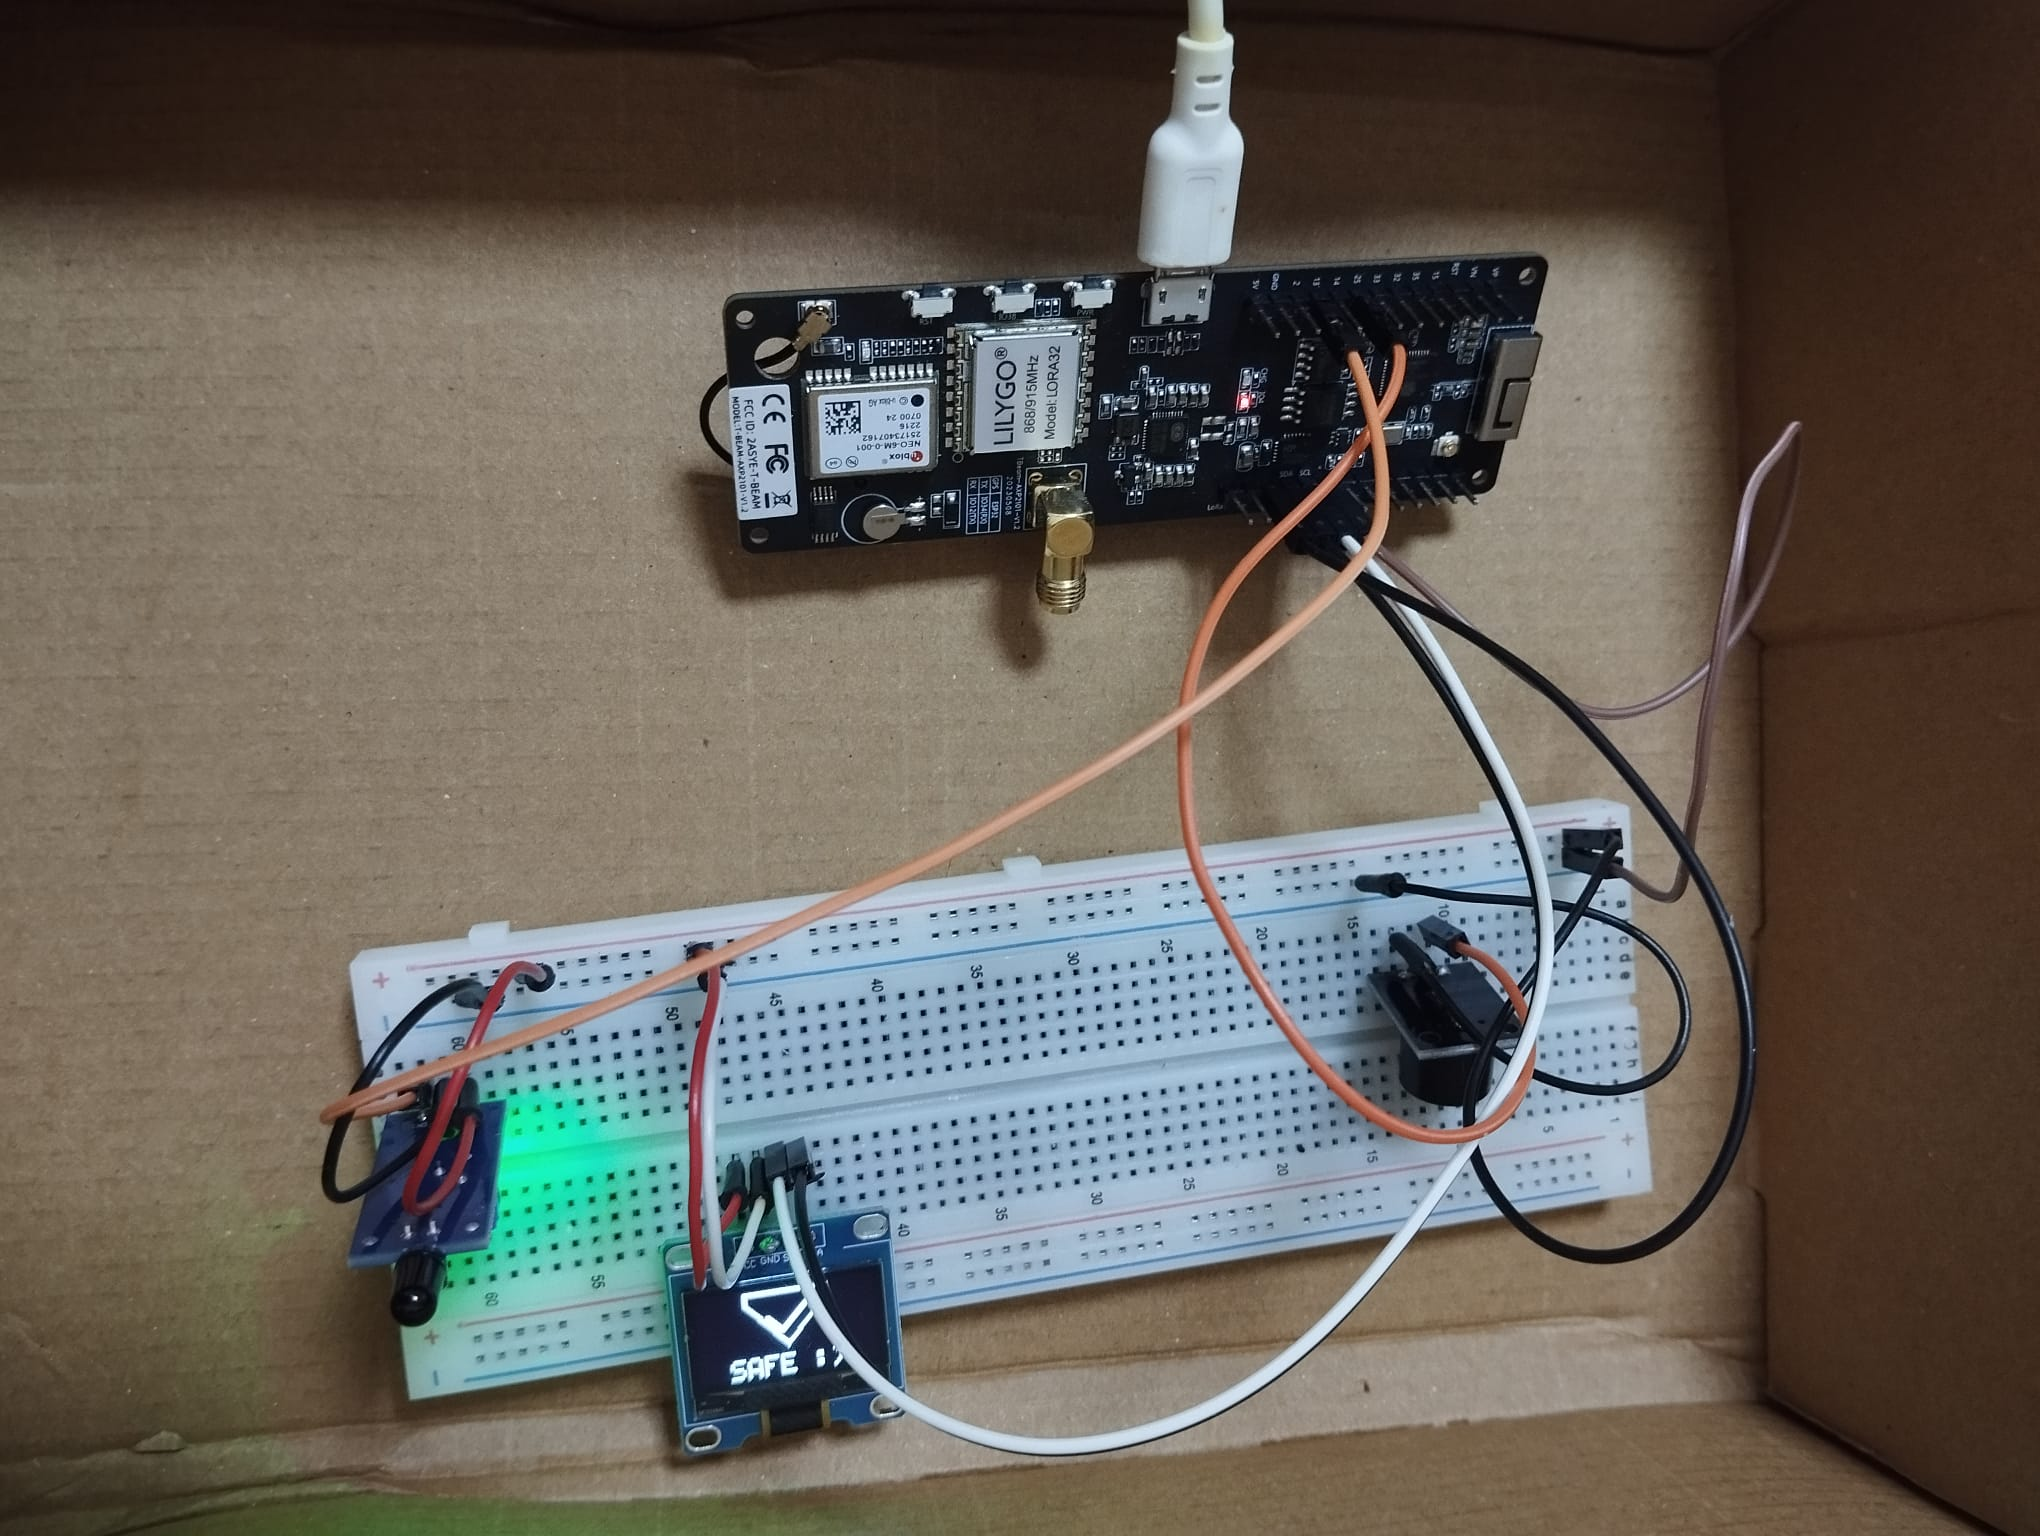
\includegraphics[width=0.56\textwidth]{all-project.jpg}

\vfill

{\large
\begin{tabular}{rl}
\textbf{University}  & Recep Tayyip Erdoğan University\\[5pt]
\textbf{Department}  & Computer Engineering\\[5pt]
\textbf{Instructor}  & Joseph Bamidele Awotunde\\[5pt]
\textbf{Name}        & Yasin ENİŞ\\[5pt]
\textbf{Student No}  & 221401043\\[5pt]
\textbf{E-mail}      & \texttt{yasin\_enis22@erdogan.edu.tr}\\[5pt]
\textbf{Platform}    & LilyGO TTGO T-Beam (ESP32), ESP-IDF (C)\\[5pt]
\end{tabular}
}

\vspace{0.9cm}
{\large \today\par}
\end{titlepage}

% ============================================================================
%  ABSTRACT + TABLE OF CONTENTS
% ============================================================================
\begin{abstract}
\noindent This report describes a real-time \textbf{flame (fire) detection and remote
monitoring} system built on a LilyGO TTGO T-Beam (ESP32) development board. The system
continuously monitors the signal from an infrared flame sensor; when a flame is
detected, it raises both an \textbf{audible} (active buzzer) and a \textbf{visual}
(SSD1306 OLED display) alert locally. At the same time, the device broadcasts its status
data over Wi-Fi using \textbf{WebSocket}, and a web control panel displays this data live:
alarm status, power/battery, signal strength, uptime, alarm-history charts, an event log,
and remote commands (mute / test / restart). All hardware components used in the project
are introduced with photographs, their technical specifications are explained, and the
wiring scheme, software architecture, and web interface are covered in detail.
\end{abstract}

\vspace{0.5cm}
\tableofcontents
\newpage

% ============================================================================
%  1. INTRODUCTION
% ============================================================================
\section{Introduction}

Fires are emergencies in which loss of life and property can be largely prevented when
they are detected early. The goal of this project is to develop a flame detection system
that provides an \textbf{early warning} using low-cost, widely available components, while
also being \textbf{remotely monitorable over a network}.

Whereas traditional smoke/flame detectors only produce a local alarm, this system adopts
an Internet of Things (IoT) approach: the device continuously streams its measured state
to a web panel. As a result, even when the user is not physically next to the device, they
can instantly view the alarm status, the device's health (battery, power source, signal
strength, memory), and the history of past alarms; and they can send remote commands.

\subsection{Key Features}
\begin{itemize}[leftmargin=1.4em]
  \item \textbf{Real-time flame detection:} The infrared flame sensor detects the IR
        radiation emitted by fire (GPIO13 digital input).
  \item \textbf{Audible alert:} The active buzzer (GPIO25) is triggered the instant a
        flame appears.
  \item \textbf{Visual alert:} The OLED shows a ``Shield (SAFE)'' icon normally and a
        full-screen ``Flame (FIRE!)'' icon during an alarm (pixel-level drawing via a
        framebuffer).
  \item \textbf{Power management:} The AXP-series PMU on the T-Beam is configured over
        I\textsuperscript{2}C; battery voltage/current and USB status are read.
  \item \textbf{Live web panel:} Status streaming, alarm-history charts, an event log, and
        remote control via WebSocket (primary) + HTTP polling (fallback).
\end{itemize}

% ============================================================================
%  2. SYSTEM ARCHITECTURE
% ============================================================================
\section{System Architecture}

The system consists of two main layers: (1) the embedded device in the field (the T-Beam
based sensor node) and (2) the web monitoring panel running in the user's browser. The
device manages the sensor and peripherals over I\textsuperscript{2}C and GPIO, and
transmits its measured state to the panel in JSON form over Wi-Fi.

\begin{figure}[H]
\centering
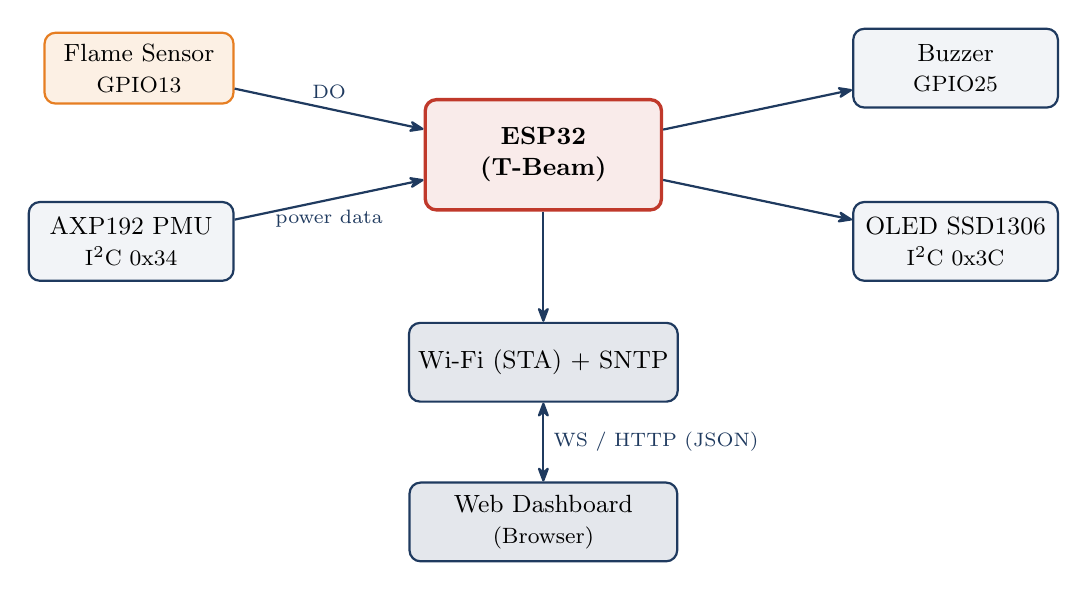
\begin{tikzpicture}[
    >={Stealth[round]},
    box/.style={rectangle, rounded corners, draw=deepblue, thick,
                minimum height=1.0cm, minimum width=2.6cm, align=center,
                fill=lightgray, font=\small},
    sensor/.style={rectangle, rounded corners, draw=flameorange, thick,
                minimum height=0.9cm, minimum width=2.4cm, align=center,
                fill=flameorange!12, font=\small},
    mcu/.style={rectangle, rounded corners, draw=flamered, very thick,
                minimum height=1.4cm, minimum width=3.0cm, align=center,
                fill=flamered!10, font=\small\bfseries},
    line/.style={->, thick, deepblue}
  ]
  % Central MCU
  \node[mcu] (mcu) {ESP32\\(T-Beam)};

  % Left: sensors / inputs
  \node[sensor] (flame) [left=2.4cm of mcu, yshift=1.1cm] {Flame Sensor\\\footnotesize GPIO13};
  \node[box]    (axp)   [left=2.4cm of mcu, yshift=-1.1cm] {AXP192 PMU\\\footnotesize I\textsuperscript{2}C 0x34};

  % Right: outputs
  \node[box] (buzzer) [right=2.4cm of mcu, yshift=1.1cm] {Buzzer\\\footnotesize GPIO25};
  \node[box] (oled)   [right=2.4cm of mcu, yshift=-1.1cm] {OLED SSD1306\\\footnotesize I\textsuperscript{2}C 0x3C};

  % Bottom: network and panel
  \node[box, fill=deepblue!12] (wifi)  [below=1.4cm of mcu] {Wi-Fi (STA) + SNTP};
  \node[box, fill=deepblue!12, minimum width=3.4cm] (panel) [below=1.0cm of wifi] {Web Dashboard\\\footnotesize (Browser)};

  % Connections
  \draw[line] (flame) -- (mcu) node[midway, above, font=\scriptsize] {DO};
  \draw[line] (axp) -- (mcu) node[midway, below, font=\scriptsize] {power data};
  \draw[line] (mcu) -- (buzzer);
  \draw[line] (mcu) -- (oled);
  \draw[line] (mcu) -- (wifi);
  \draw[line, <->] (wifi) -- (panel) node[midway, right, font=\scriptsize] {WS / HTTP (JSON)};
\end{tikzpicture}
\caption{System block diagram: sensor input, peripheral outputs, and the network layer.}
\label{fig:arch}
\end{figure}

\noindent The actual assembly of the device is shown in Figure~\ref{fig:montaj}; the
T-Beam board is connected with jumper wires to the sensor, buzzer, and OLED on the
breadboard.

\begin{figure}[H]
\centering
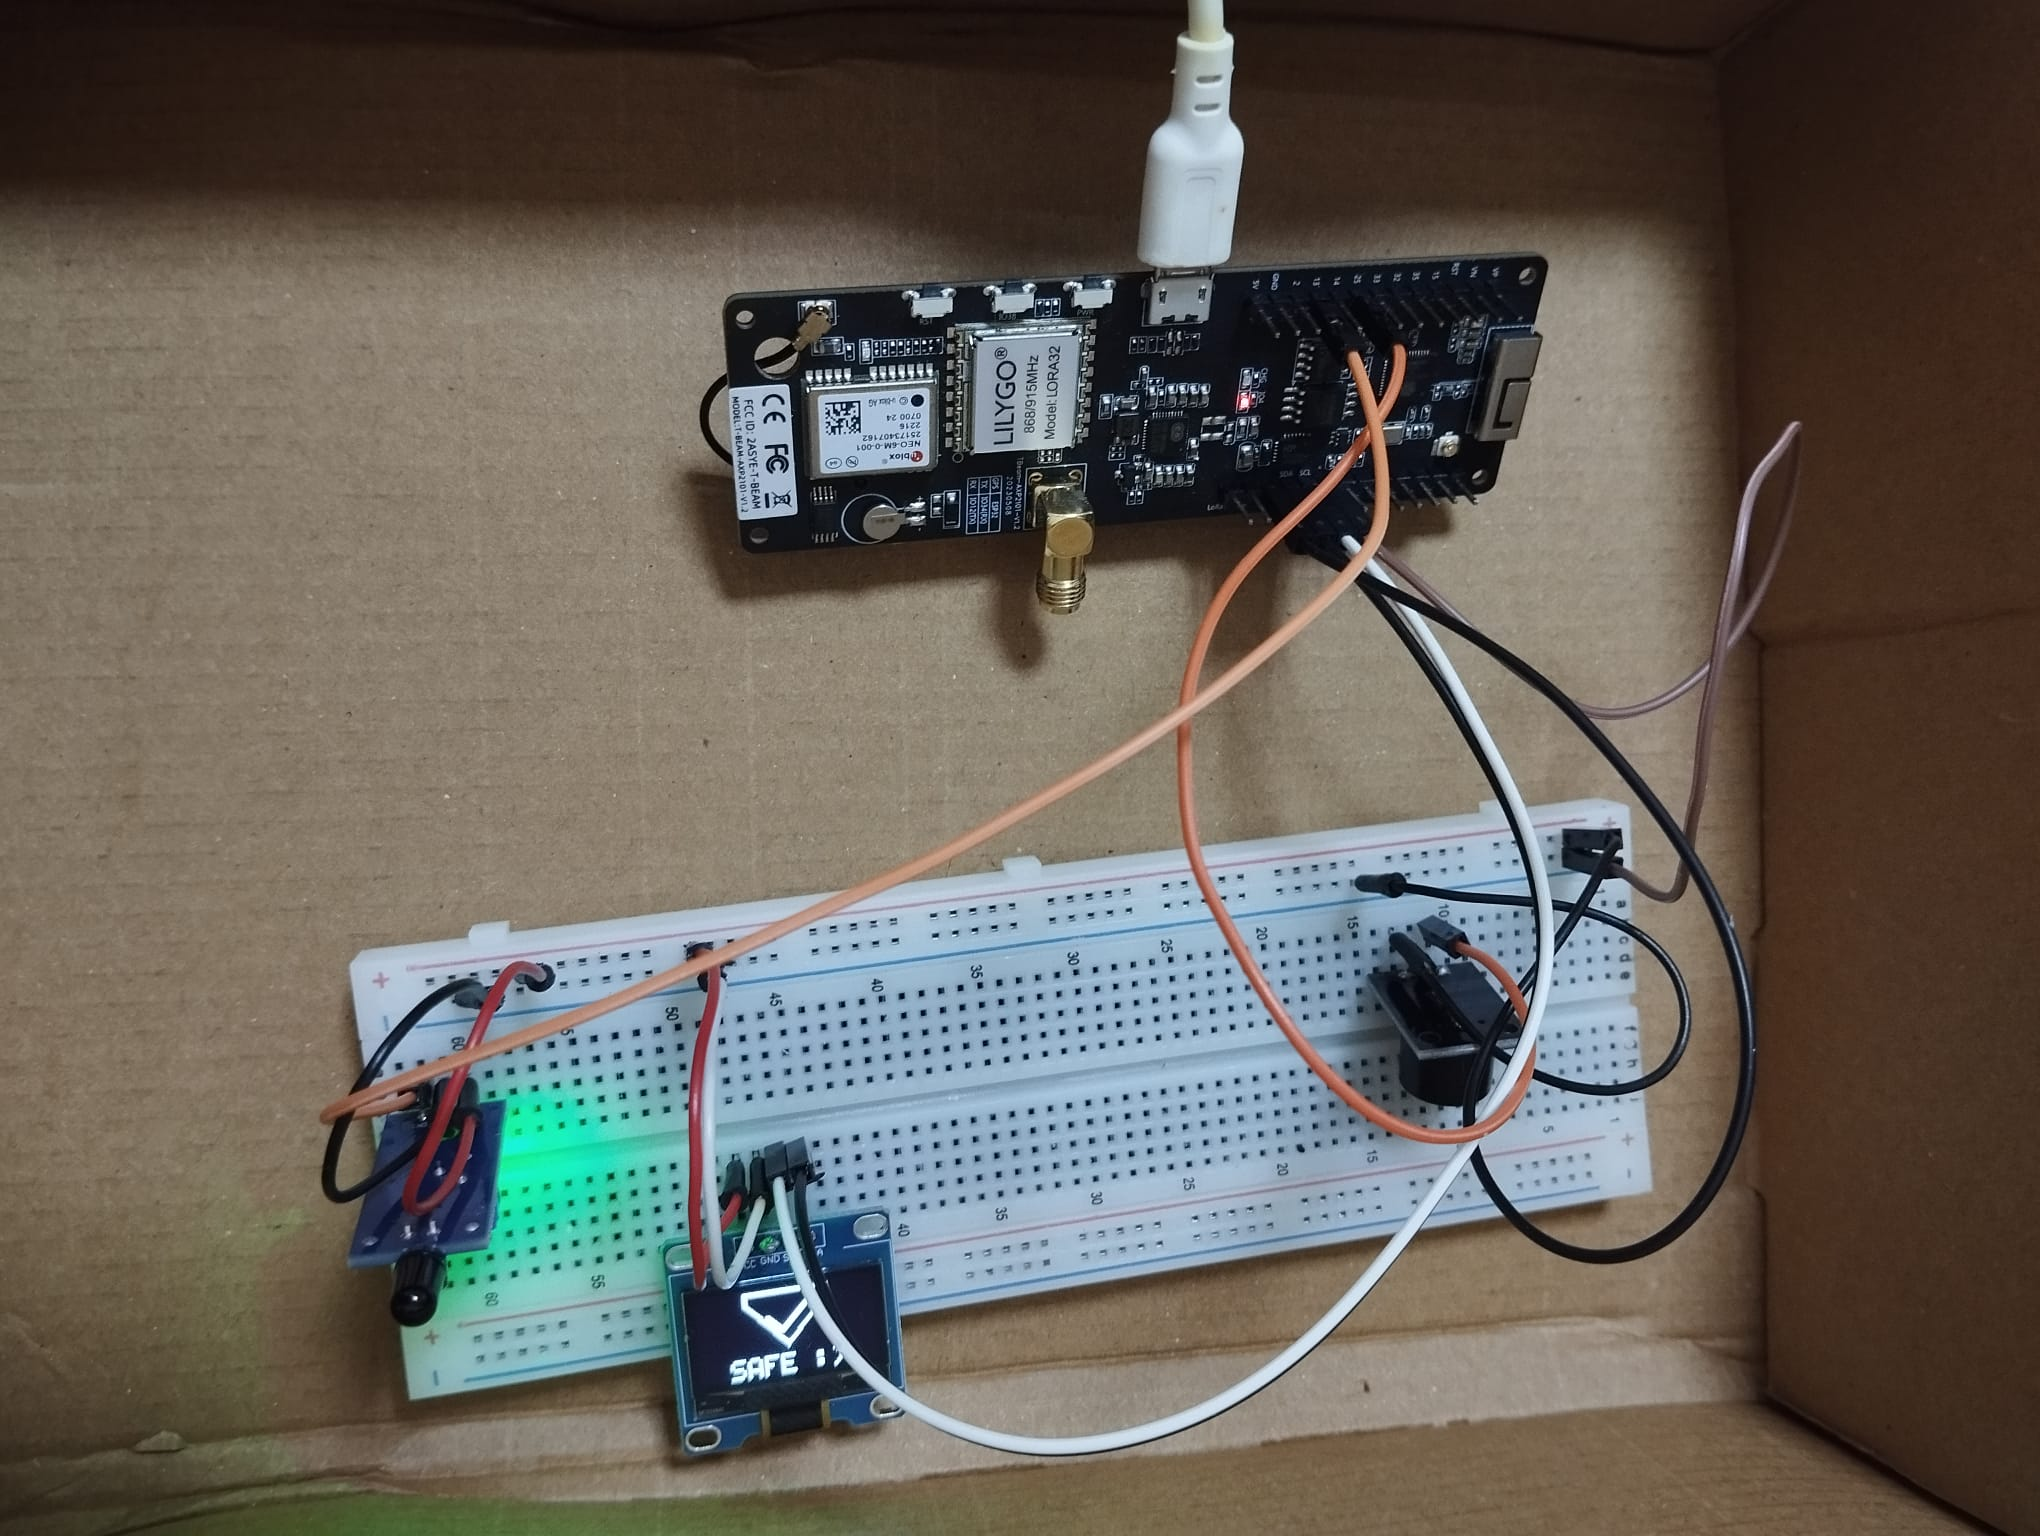
\includegraphics[width=0.78\textwidth]{all-project.jpg}
\caption{The completed system assembled on the breadboard. The OLED display shows the
``SAFE'' state.}
\label{fig:montaj}
\end{figure}

% ============================================================================
%  3. HARDWARE COMPONENTS
% ============================================================================
\section{Hardware Components}

This section introduces each component used in the system with a photograph and explains
its technical specifications and its role in the project.

% ---------------------------------------------------------------------------
\subsection{LilyGO TTGO T-Beam (ESP32 Development Board)}

\begin{figure}[H]
\centering
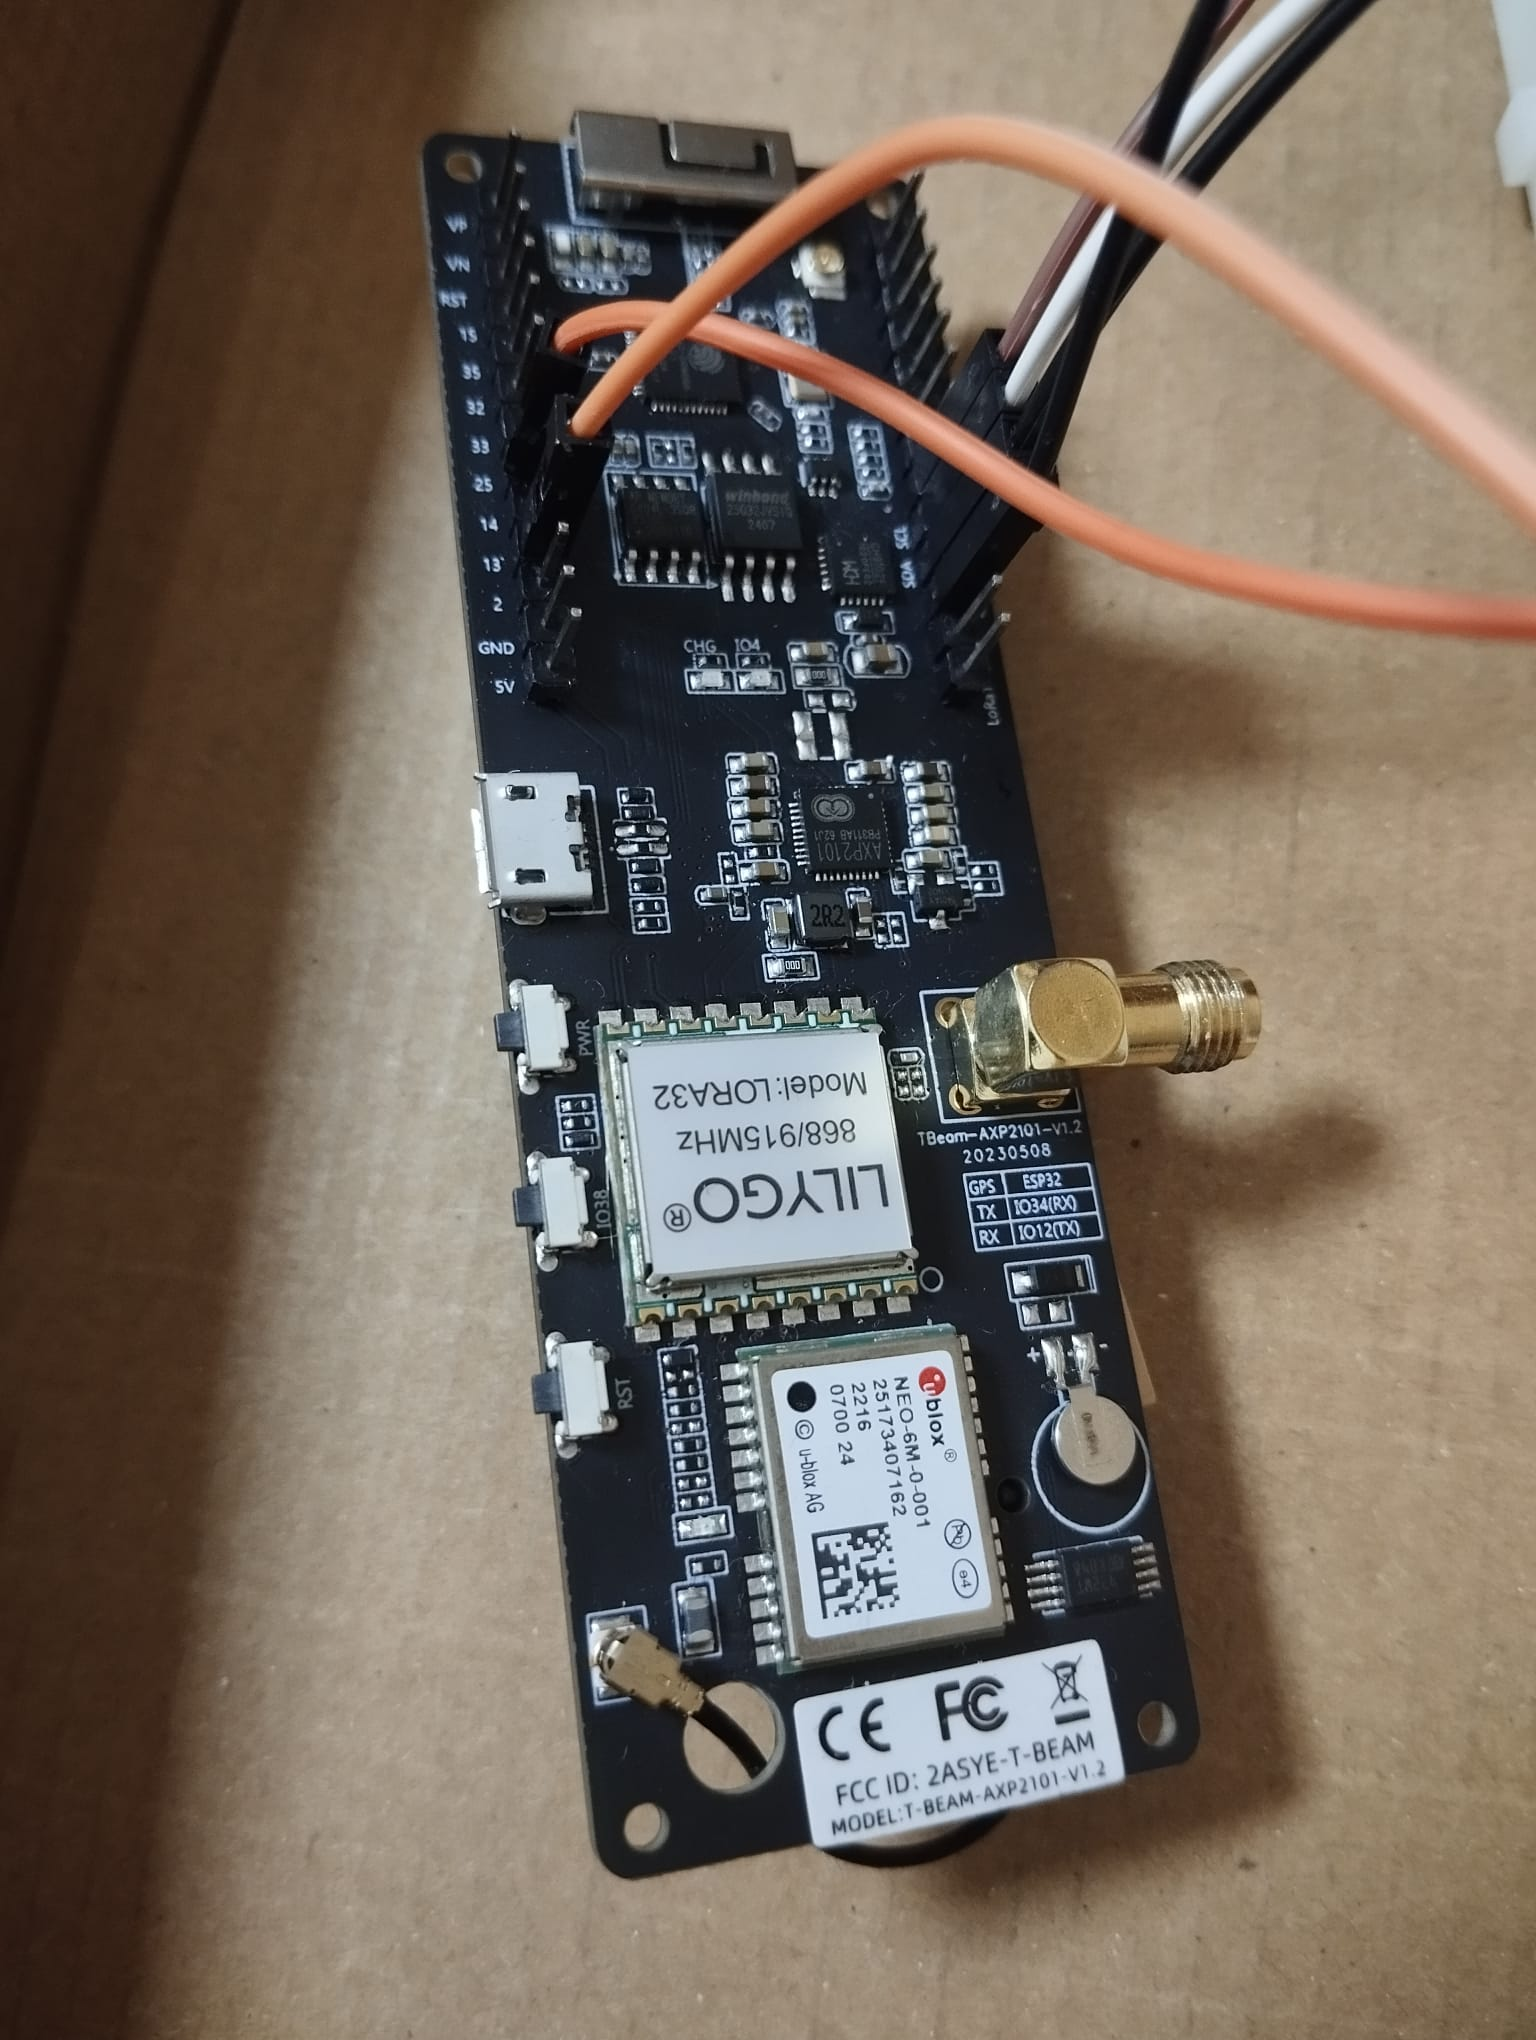
\includegraphics[width=0.42\textwidth]{t-beam.jpg}
\caption{LilyGO TTGO T-Beam development board (ESP32 + LoRa + GPS + AXP PMU).}
\label{fig:tbeam}
\end{figure}

The brain of the project, the T-Beam, is a versatile development board carrying the
Espressif \textbf{ESP32} processor. It includes several integrated units for
communication and power management.

\begin{table}[H]
\centering
\caption{LilyGO TTGO T-Beam technical specifications.}
\begin{tabular}{L{4.2cm} L{9.5cm}}
\toprule
\textbf{Feature} & \textbf{Description}\\
\midrule
Processor (MCU)    & Espressif ESP32, dual-core Xtensa LX6, up to 240 MHz\\
Wireless           & Wi-Fi 802.11 b/g/n + Bluetooth / BLE (integrated)\\
LoRa Module        & Semtech SX127x based (868/915 MHz), with SMA antenna input\\
GPS                & u-blox NEO-6M GNSS receiver\\
Power Mgmt. (PMU)  & AXP-series PMU (firmware uses the AXP192 register map, I\textsuperscript{2}C 0x34)\\
Battery            & 18650 Li-ion holder on the back, built-in charging circuit\\
Interface          & Micro-USB (power + programming), numerous GPIOs\\
\bottomrule
\end{tabular}
\end{table}

\noindent\textbf{Role in the project:} This project uses the T-Beam's \textbf{ESP32 core},
its \textbf{Wi-Fi}, its \textbf{GPIOs}, the \textbf{I\textsuperscript{2}C} bus, and its
\textbf{AXP192 PMU}. The PMU turns on the 3.3V power rails (LDO2/LDO3) that supply the
OLED and provides battery/power telemetry. The LoRa and GPS units are not used in this
project; they are left as potential future extensions.

% ---------------------------------------------------------------------------
\subsection{Infrared Flame Sensor}

\begin{figure}[H]
\centering
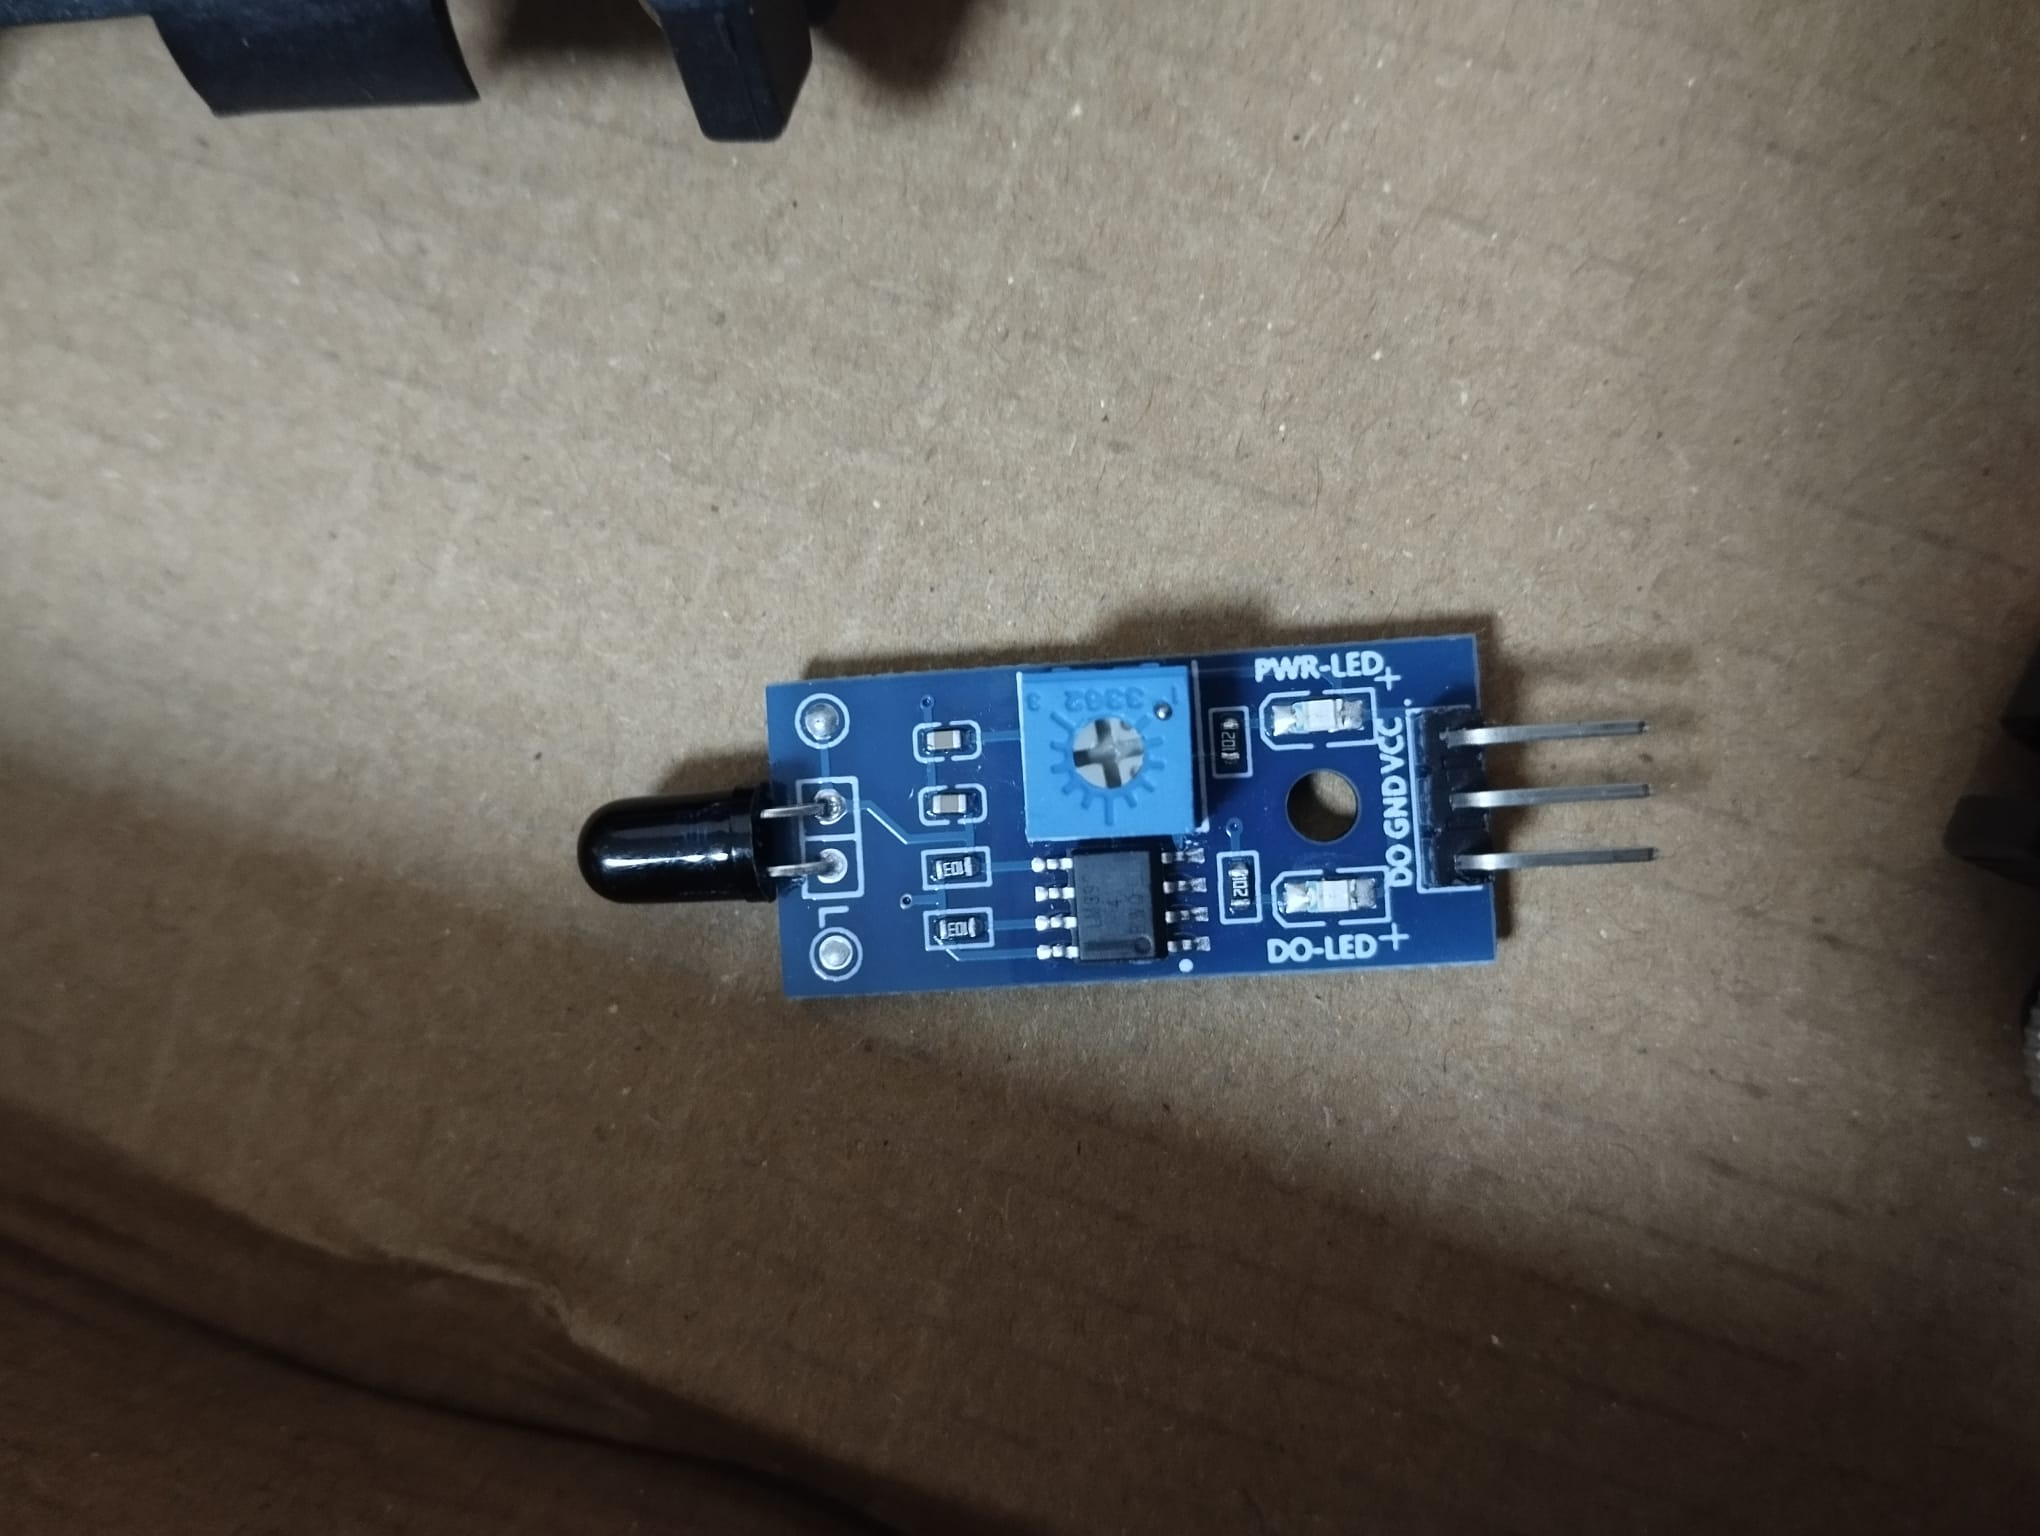
\includegraphics[width=0.55\textwidth]{flame-sensor.jpg}
\caption{Infrared (IR) flame sensor module; the black IR receiver, the LM393 comparator,
and the sensitivity-adjustment potentiometer.}
\label{fig:flame}
\end{figure}

The flame sensor contains a photodiode that detects infrared radiation around 760--1100~nm
emitted by fire. The LM393 comparator on the module compares this radiation against a
threshold to produce a clean digital signal.

\begin{table}[H]
\centering
\caption{Flame sensor module specifications.}
\begin{tabular}{L{4.2cm} L{9.5cm}}
\toprule
\textbf{Feature} & \textbf{Description}\\
\midrule
Detection principle & IR photodiode (sensitive to flame radiation, $\sim$760--1100 nm)\\
Comparator          & LM393 (op-amp comparator)\\
Outputs             & Digital (DO) and Analog (AO)\\
Sensitivity adjust  & Threshold set via the on-board potentiometer\\
Detection angle     & within a $\sim$60$^\circ$ cone\\
Supply              & 3.3V -- 5V\\
Indicators          & Power LED (PWR) and digital-output LED (DO)\\
\bottomrule
\end{tabular}
\end{table}

\noindent\textbf{Role in the project:} The sensor's \textbf{digital output (DO)} is
connected to the T-Beam's \textbf{GPIO13} pin. The firmware reads this pin every 200~ms;
when a flame is detected, the output goes \textbf{LOW (0)} and the system enters the alarm
state. The analog output (AO) is not used in this project.

% ---------------------------------------------------------------------------
\subsection{HW-508 Active Buzzer Module}

\begin{figure}[H]
\centering
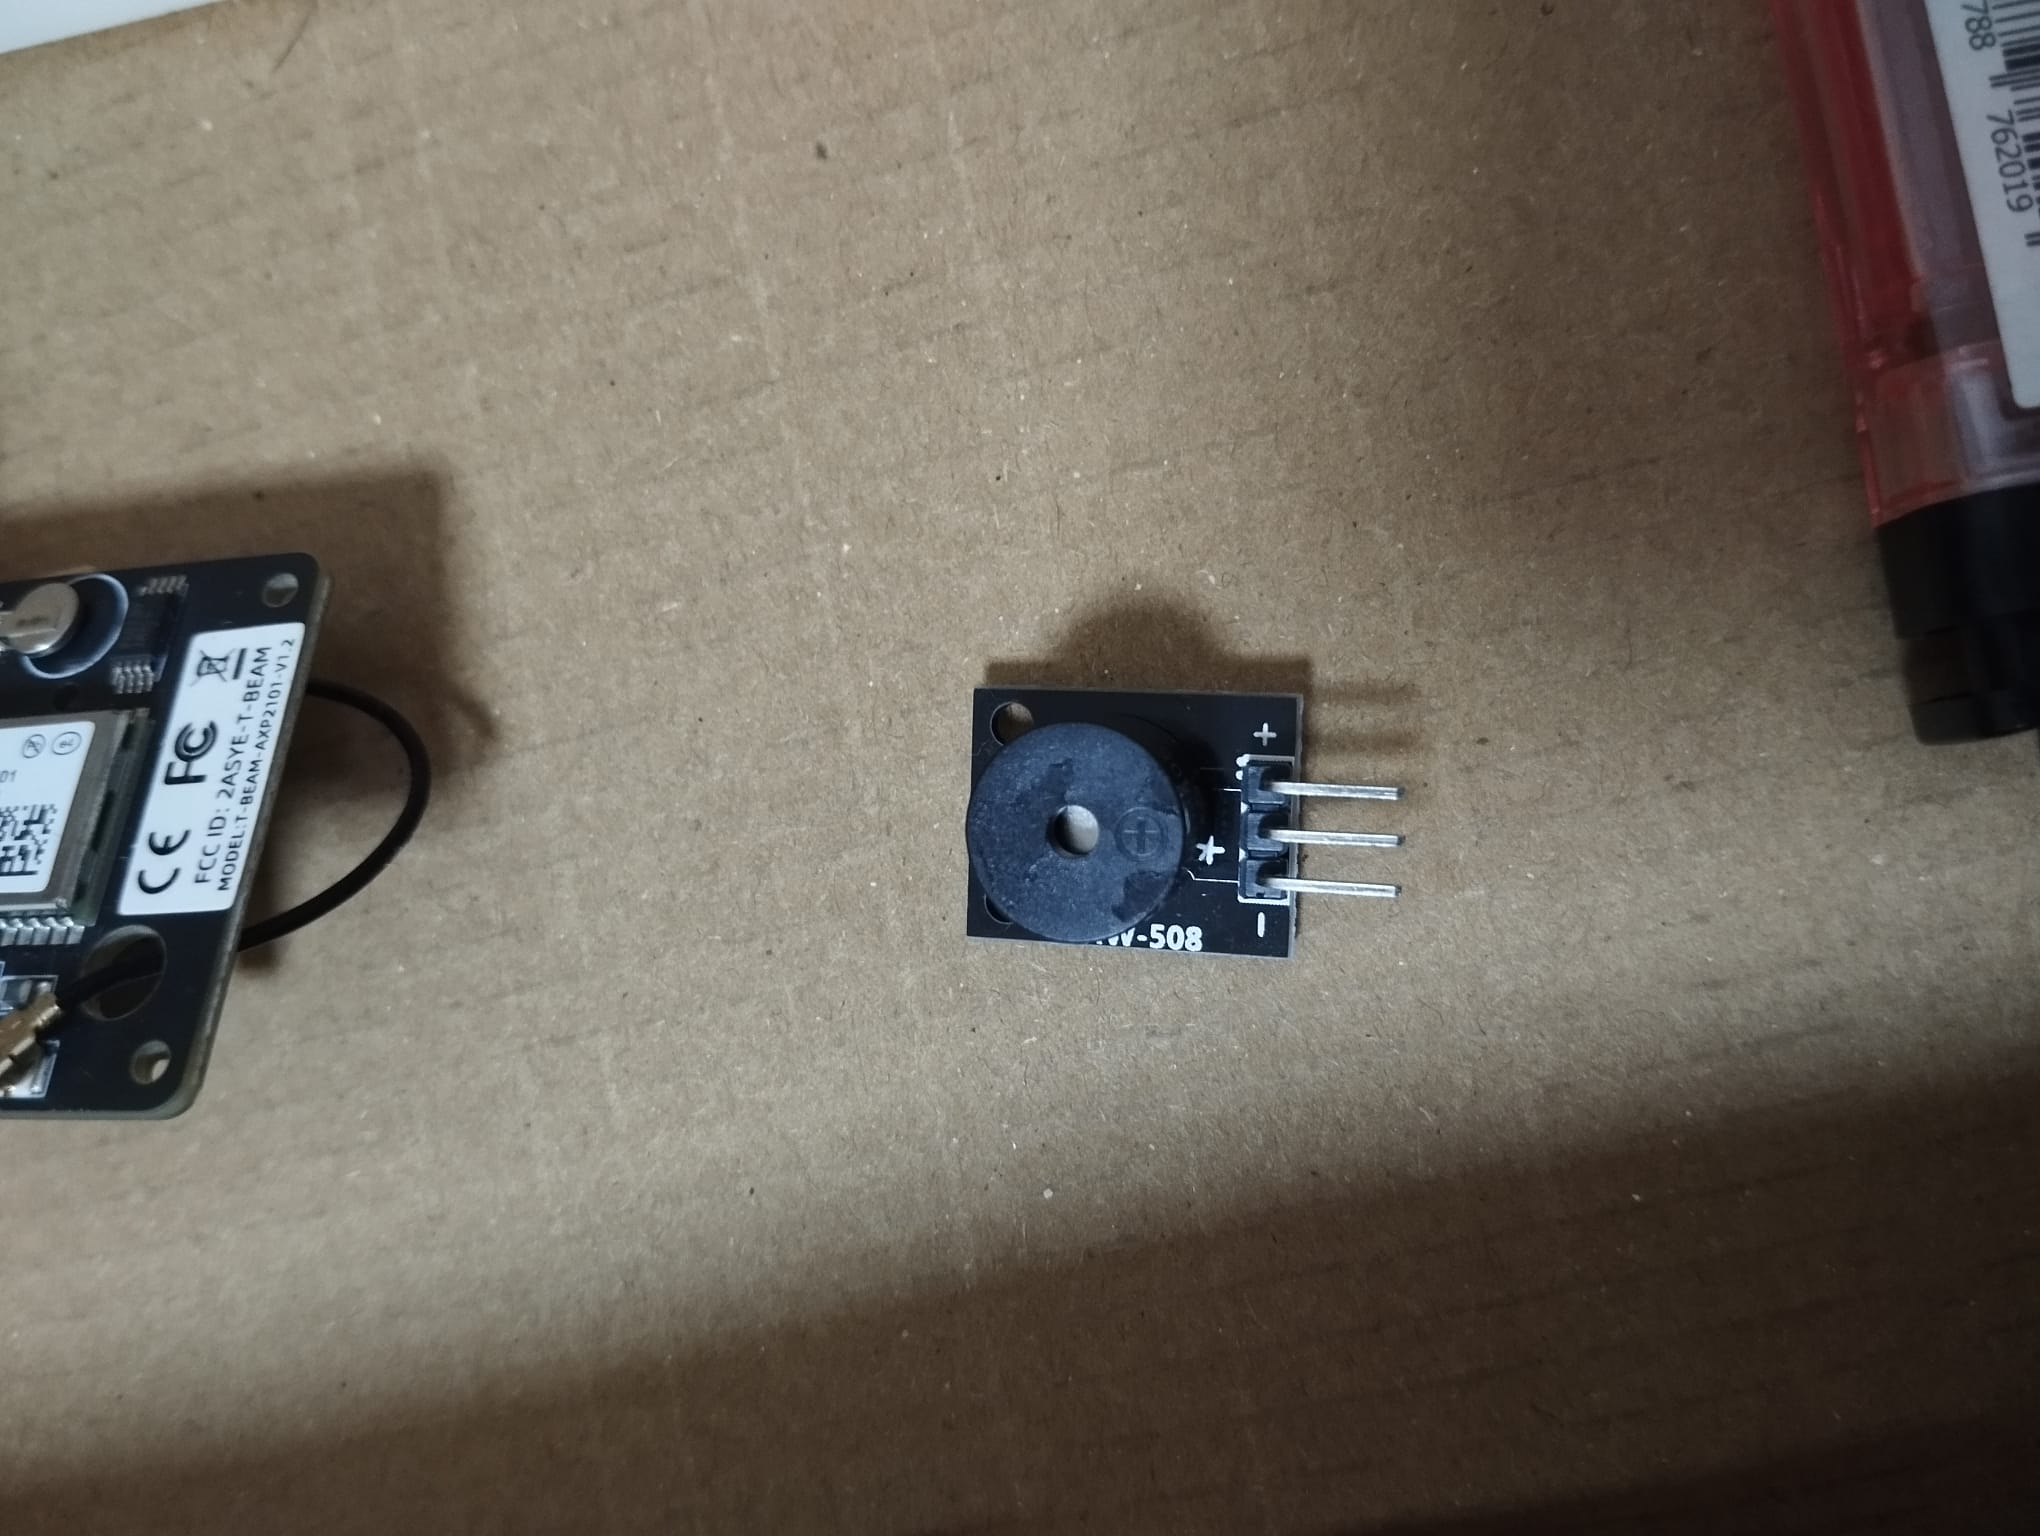
\includegraphics[width=0.55\textwidth]{buzzer.jpg}
\caption{HW-508 active buzzer module.}
\label{fig:buzzer}
\end{figure}

The HW-508 is an \textbf{active} buzzer module with its own internal oscillator. Because of
this, no PWM/frequency signal is needed to produce sound; it simply sounds when supplied
with power.

\begin{table}[H]
\centering
\caption{HW-508 active buzzer specifications.}
\begin{tabular}{L{4.2cm} L{9.5cm}}
\toprule
\textbf{Feature} & \textbf{Description}\\
\midrule
Type            & Active buzzer (built-in oscillator)\\
Drive           & DC supply is sufficient; no PWM required\\
Operating voltage & $\sim$3.3V -- 5V\\
Pins            & (+) VCC, (--) GND, (S/I) signal\\
\bottomrule
\end{tabular}
\end{table}

\noindent\textbf{Role in the project:} On this module, to avoid a continuous-beeping issue,
the \textbf{VCC pin is connected directly to GPIO25} (active-high drive). When the ESP32
drives GPIO25 \textbf{HIGH}, power reaches the buzzer and it sounds; when \textbf{LOW}, it
goes silent. The signal (S/I) pin is left unconnected. This way the buzzer can be
controlled directly by the flame state (and by the ``mute'' command).

% ---------------------------------------------------------------------------
\subsection{0.96" OLED Display (SSD1306)}

\begin{figure}[H]
\centering
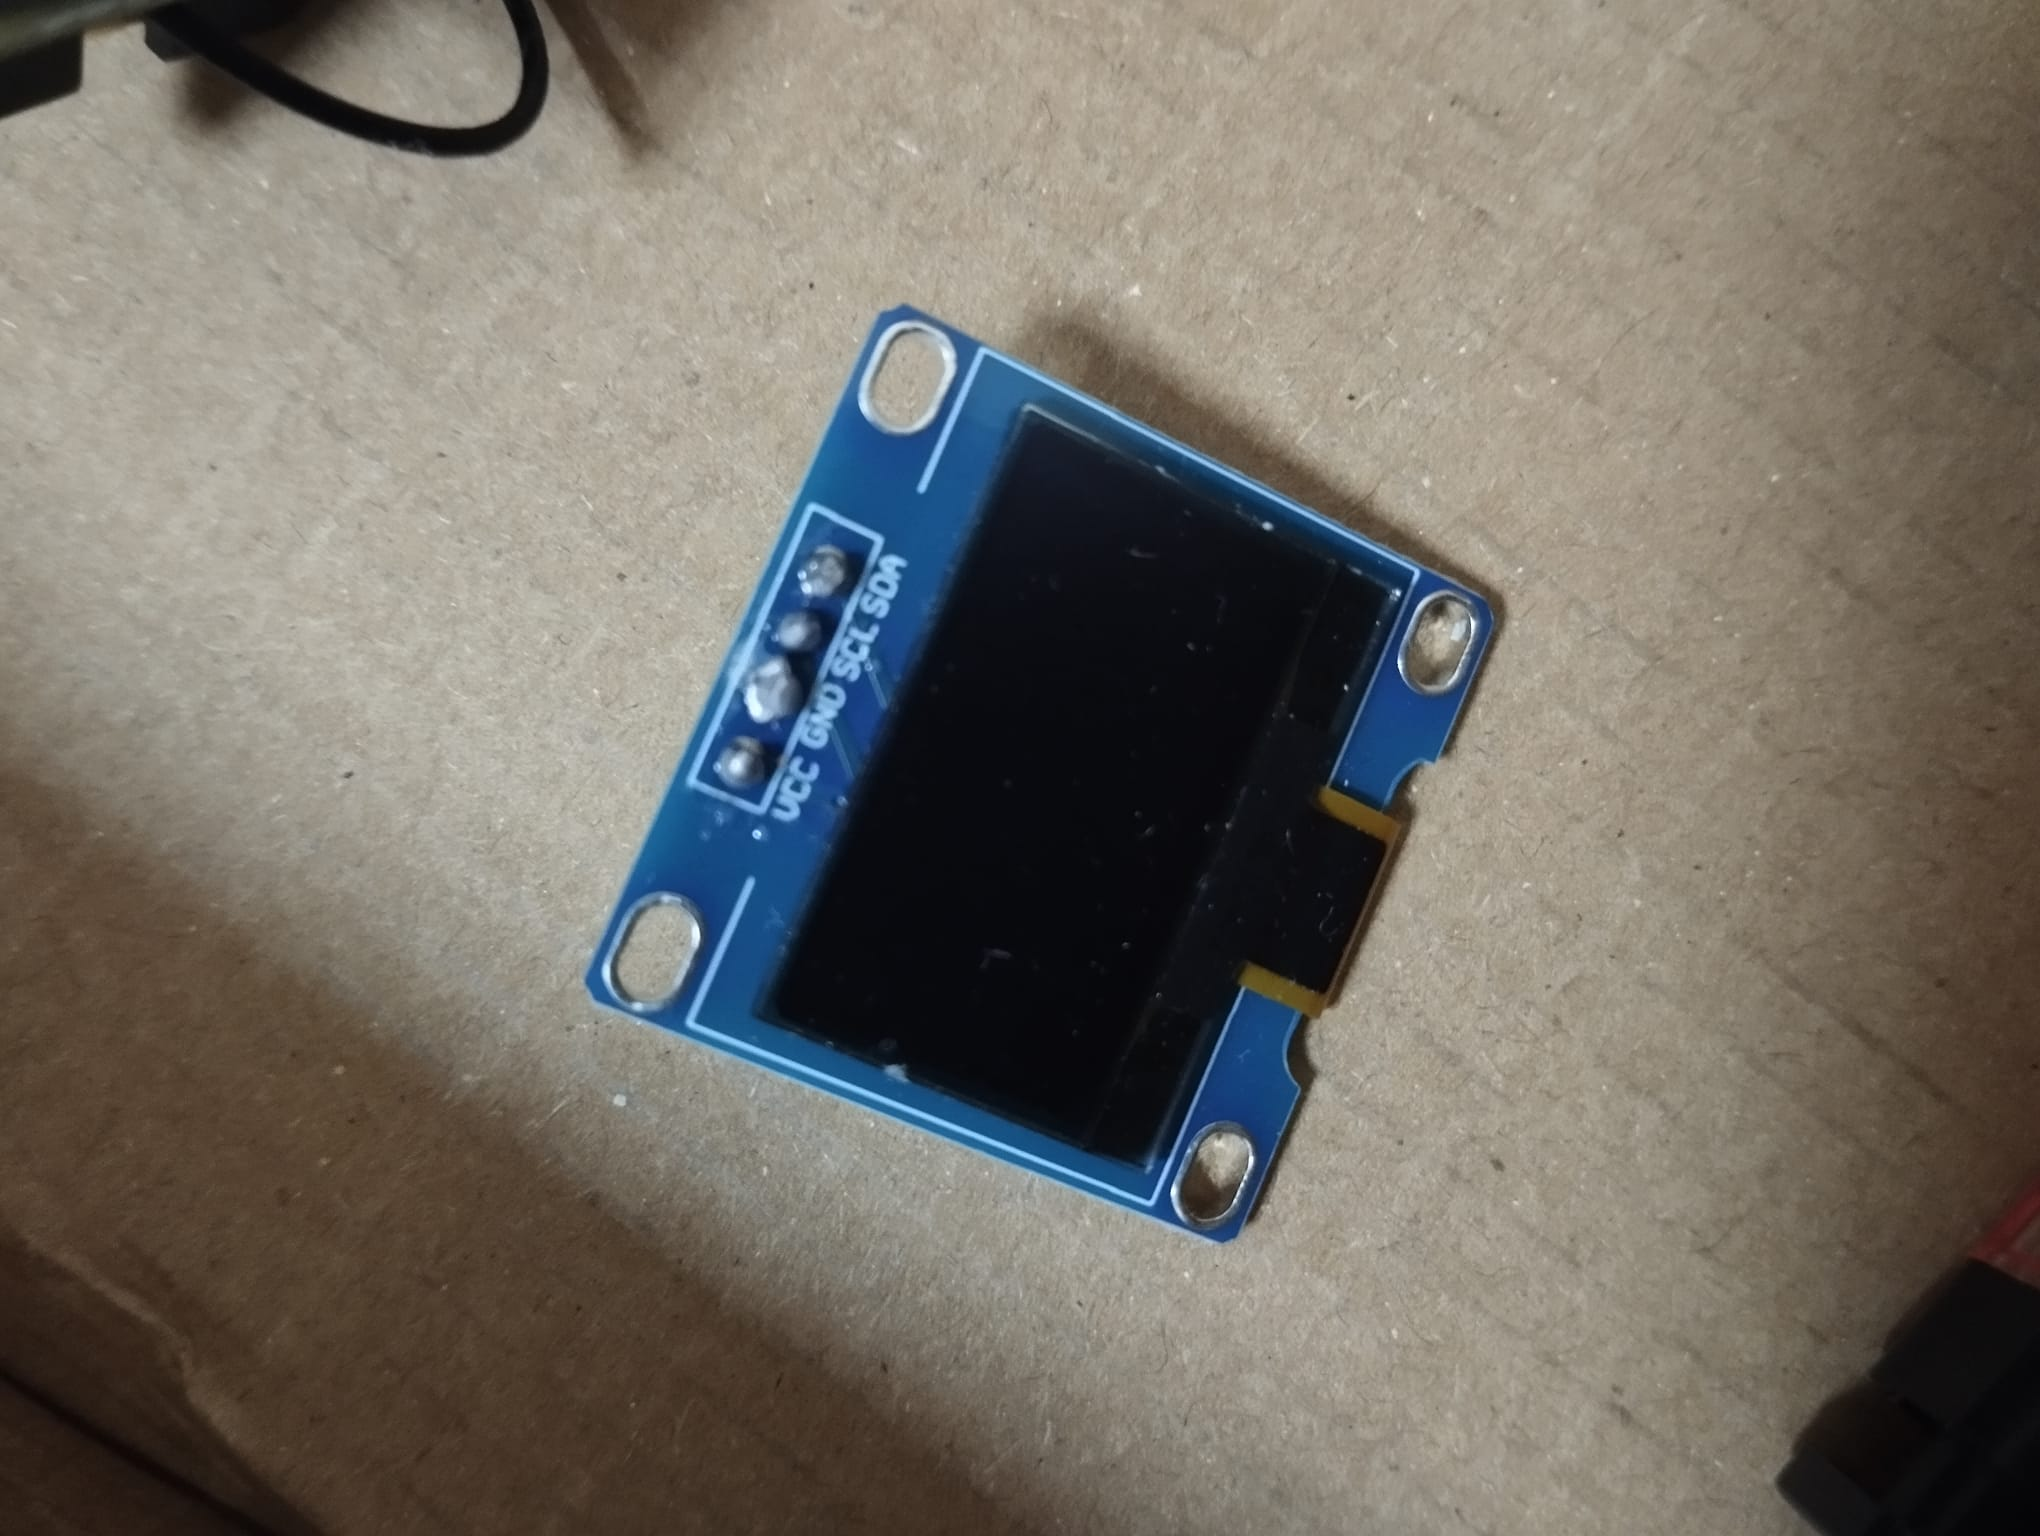
\includegraphics[width=0.55\textwidth]{oled-display.jpg}
\caption{0.96-inch I\textsuperscript{2}C OLED display (SSD1306, 128$\times$64 pixels).}
\label{fig:oled}
\end{figure}

This OLED display with an SSD1306 driver is a self-illuminating (no backlight required),
high-contrast monochrome display and is driven with just four wires (I\textsuperscript{2}C).

\begin{table}[H]
\centering
\caption{OLED display specifications.}
\begin{tabular}{L{4.2cm} L{9.5cm}}
\toprule
\textbf{Feature} & \textbf{Description}\\
\midrule
Diagonal / resolution & 0.96 inch / 128$\times$64 pixels\\
Driver               & SSD1306\\
Interface            & I\textsuperscript{2}C (4 pins: VCC, GND, SCL, SDA)\\
I\textsuperscript{2}C address & 0x3C\\
Supply               & 3.3V -- 5V\\
Technology           & OLED (self-illuminating, high contrast)\\
\bottomrule
\end{tabular}
\end{table}

\noindent\textbf{Role in the project:} The display is connected to the T-Beam's
I\textsuperscript{2}C bus (\textbf{SDA=GPIO21}, \textbf{SCL=GPIO22}). By drawing pixel by
pixel into a 1024-byte \textbf{framebuffer}, the firmware produces two full-screen icons: a
``Shield + Check (SAFE)'' in the normal state and a ``Flame (FIRE!)'' during an alarm. The
drawings are precomputed and pushed to the screen in a single transfer.

% ============================================================================
%  4. WIRING SCHEME
% ============================================================================
\section{Wiring Scheme}

All components share the common 3.3V power and GND rails over the breadboard.
Table~\ref{tab:pin} summarizes each component's connection to the T-Beam.

\begin{table}[H]
\centering
\caption{Pin connection table.}
\label{tab:pin}
\begin{tabular}{L{3.2cm} L{2.0cm} L{4.0cm} L{4.0cm}}
\toprule
\textbf{Component} & \textbf{Pin} & \textbf{T-Beam Connection} & \textbf{Note}\\
\midrule
Flame Sensor & VCC & 3.3V & --\\
             & GND & GND & --\\
             & DO  & GPIO13 (INPUT) & Digital signal; flame = LOW\\
             & AO  & Unused & Not used\\
\addlinespace
HW-508 Buzzer & (+) VCC & GPIO25 (OUTPUT) & Active-high; HIGH = sounds\\
              & (--) GND & GND & --\\
              & S / I   & Unused & Not used\\
\addlinespace
OLED (SSD1306) & VCC & 3.3V & via AXP192 LDO2\\
               & GND & GND & --\\
               & SDA & GPIO21 & I\textsuperscript{2}C data\\
               & SCL & GPIO22 & I\textsuperscript{2}C clock\\
\bottomrule
\end{tabular}
\end{table}

\noindent\textbf{Important note:} The VCC pin of the HW-508 active buzzer is connected
directly to GPIO25, \emph{not} to the 3.3V rail. This way the buzzer's power is switched
directly by the GPIO and unwanted continuous beeping is prevented.

% ============================================================================
%  5. SOFTWARE / FIRMWARE
% ============================================================================
\section{Software (Firmware)}

The device firmware was developed in \textbf{C} using \textbf{ESP-IDF} (Espressif IoT
Development Framework). The application runs on FreeRTOS and has a modular structure.

\subsection{General Operation Flow}
At startup, the I\textsuperscript{2}C bus, the AXP192 PMU (power rails + ADC), the OLED
display, and the GPIOs are initialized in order; then Wi-Fi (STA) and SNTP (for a real
timestamp) come up. The actual monitoring runs in a FreeRTOS task
(\texttt{monitor\_task}):

\begin{itemize}[leftmargin=1.4em]
  \item The flame sensor (GPIO13) is read every 200~ms.
  \item On a state change (safe $\leftrightarrow$ flame) the OLED is updated, a record is
        appended to the alarm history, and a WebSocket broadcast is sent \textbf{immediately}.
  \item The buzzer (GPIO25) is driven according to the flame state and the ``mute'' command.
  \item Even without a flame, a status broadcast is sent every 2~seconds to keep the panel
        ``live''.
\end{itemize}

\subsection{OLED Framebuffer Drawing}
The screen content is built pixel by pixel in a 128$\times$64 = 1024-byte buffer
(framebuffer). The ``Flame'' and ``Shield'' icons are drawn using row-by-row half-width
tables and a custom 5$\times$7 font; the ready buffer is pushed to the display in a single
transfer over I\textsuperscript{2}C.

\subsection{AXP192 Power Telemetry}
By enabling the PMU's ADC channels, the battery voltage (12-bit), the charge and discharge
current (13-bit), and the USB/charge status are read. If no battery is installed, the
voltage and percentage read 0 (this is normal). These data are reflected on the panel as
the power card.

\subsection{Network Layer and Data Contract}
When the device connects to Wi-Fi, it starts an HTTP/WebSocket server. The endpoints
consumed by the panel are:

\begin{table}[H]
\centering
\caption{Network endpoints served by the device.}
\begin{tabular}{L{5.0cm} L{9.0cm}}
\toprule
\textbf{Endpoint} & \textbf{Purpose}\\
\midrule
\texttt{ws://<IP>/ws}         & Live status broadcast + remote command (primary)\\
\texttt{GET /api/status}      & Instant status (HTTP fallback / polling)\\
\texttt{GET /api/alarms}      & Alarm history (for charts and the log)\\
\texttt{POST /api/command}    & Remote command (\texttt{mute}/\texttt{test}/\texttt{restart})\\
\bottomrule
\end{tabular}
\end{table}

\noindent The status data sent from the device to the panel conforms \emph{exactly} to the
following JSON schema:

\begin{quote}\footnotesize\ttfamily
\{\\
\hspace*{1em}"deviceId": "tbeam-01", "online": true, "timestamp": 1718560000,\\
\hspace*{1em}"uptimeSec": 38211, "firmware": "1.0.0",\\
\hspace*{1em}"flame": \{ "detected": false, "sensorActive": true \},\\
\hspace*{1em}"buzzer": false,\\
\hspace*{1em}"power": \{ "usbConnected": true, "charging": true,\\
\hspace*{2em}"batteryPercent": 87, "batteryVoltage": 4.05, "currentMa": 120 \},\\
\hspace*{1em}"wifi": \{ "rssi": -58 \},\\
\hspace*{1em}"system": \{ "freeHeap": 142000 \}\\
\}
\end{quote}

% ============================================================================
%  6. WEB DASHBOARD (GUI)
% ============================================================================
\section{Web Monitoring Panel (GUI)}

The web panel is a static application written with HTML, Tailwind CSS, and vanilla
JavaScript, using Chart.js for charts and requiring no build step. It connects to the
device via \textbf{WebSocket}; if the connection drops, it automatically falls back to
\textbf{HTTP polling}. The interface is bilingual (TR/EN) and supports dark/light themes.

\begin{figure}[H]
\centering
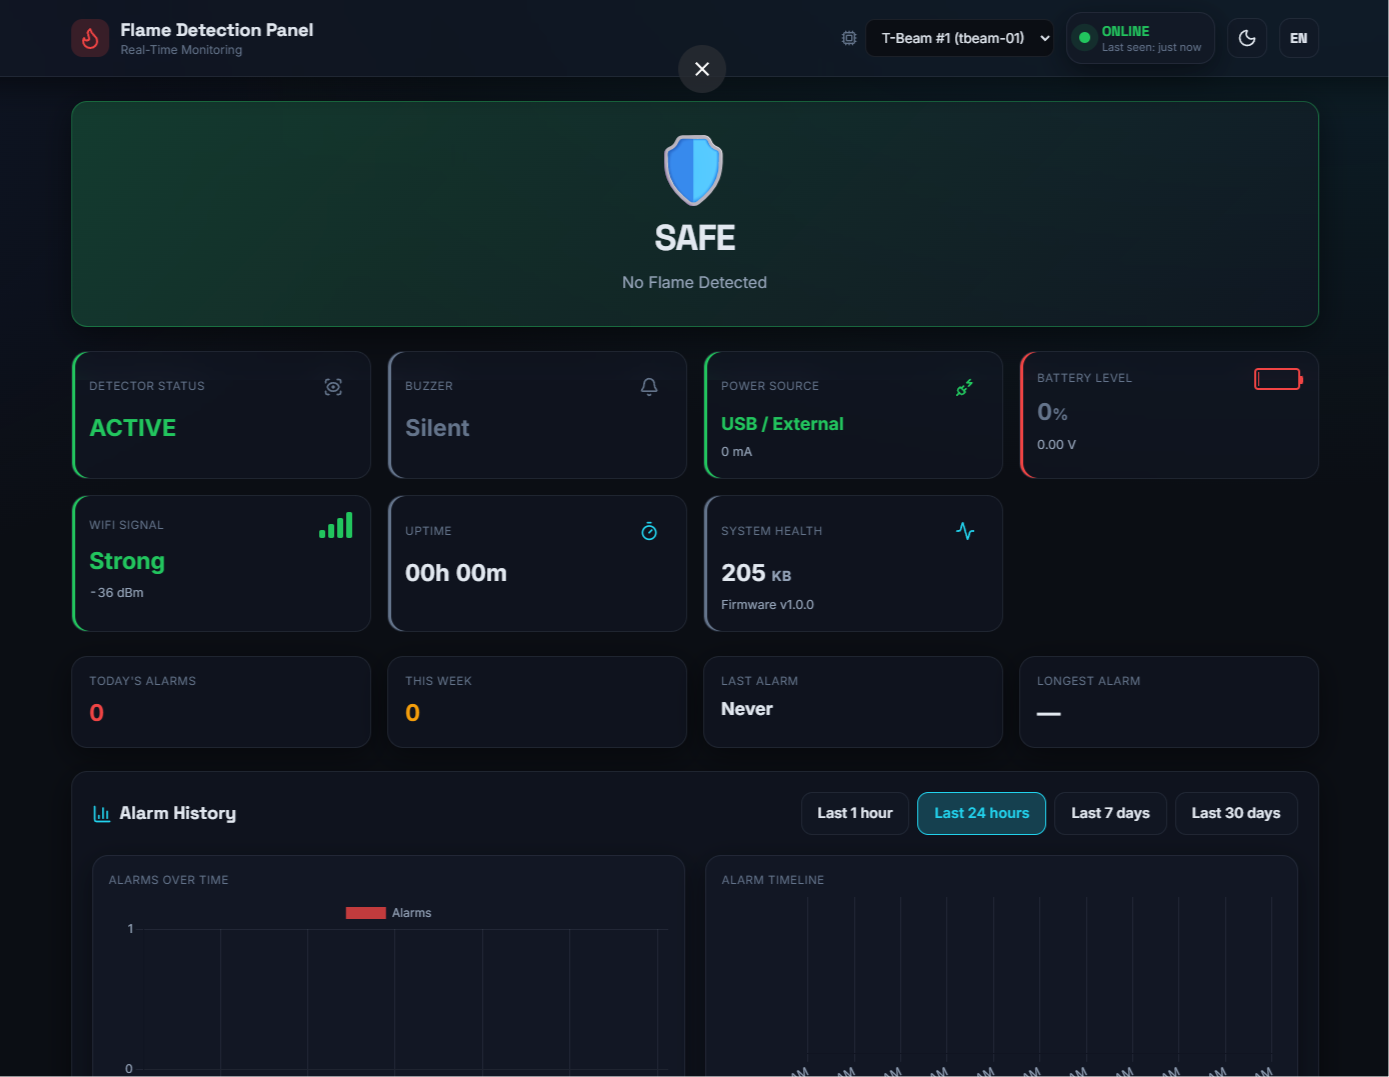
\includegraphics[width=0.92\textwidth]{dashboard.png}
\caption{The web panel in the normal (SAFE) state. The main status panel is at the top;
below it are the detector, buzzer, power source, battery, Wi-Fi signal, uptime, and system
health cards; at the bottom are the alarm-history charts.}
\label{fig:gui-safe}
\end{figure}

\noindent As shown in Figure~\ref{fig:gui-safe}, the panel presents all of the device's
telemetry at a glance. When a flame is detected, the interface switches to the
\textbf{red alarm} state in Figure~\ref{fig:gui-alarm}: the main panel shows the
``FLAME DETECTED!'' warning, the buzzer card becomes ``SOUNDING'', the screen edge pulses
red, and the audible/visual alerts are triggered.

\begin{figure}[H]
\centering
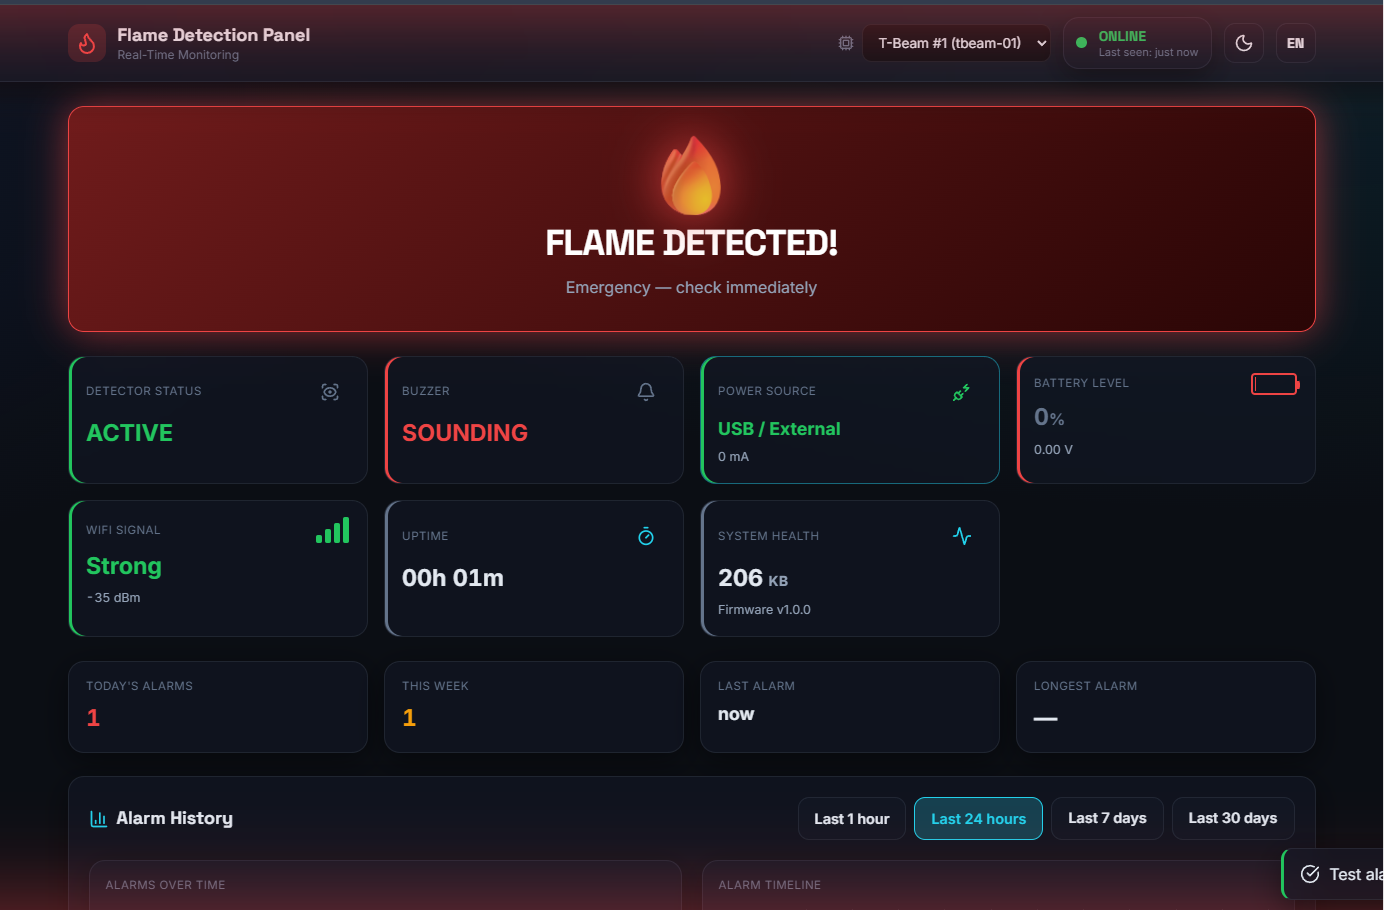
\includegraphics[width=0.92\textwidth]{dashboard-alarm.png}
\caption{The web panel in the alarm (FLAME DETECTED) state. The buzzer is ``SOUNDING'',
the day's alarm counter has increased, and ``Last Alarm'' has been updated to the current
moment.}
\label{fig:gui-alarm}
\end{figure}

\subsection{Panel Components}
\begin{itemize}[leftmargin=1.4em]
  \item \textbf{Main alarm panel:} Safe (green shield) / Flame (red, flashing).
  \item \textbf{Status cards:} Detector, buzzer, power source, battery (voltage/charge),
        Wi-Fi (RSSI bars), uptime, system health (free memory + firmware).
  \item \textbf{Statistics cards:} Today's/weekly alarm counts, last alarm (relative time),
        longest alarm.
  \item \textbf{Charts (Chart.js):} Alarms over time, alarm timeline, battery voltage and
        signal trend (1h / 24h / 7d / 30d ranges).
  \item \textbf{Event log:} Live row insertion, CSV export, ``Acknowledge''.
  \item \textbf{Remote control:} Mute the buzzer, test alarm, restart (with a confirmation
        modal).
  \item \textbf{Offline detection:} If no data arrives for a certain time, the device is
        automatically considered ``OFFLINE'' and the interface gracefully enters a waiting
        state.
\end{itemize}

% ============================================================================
%  7. TESTING AND RESULTS
% ============================================================================
\section{Testing and Results}

The system was tested both locally and on the network side:
\begin{itemize}[leftmargin=1.4em]
  \item \textbf{Local alert:} When a flame source was brought close to the sensor, the
        buzzer sounded immediately and the OLED switched to the ``FIRE!'' icon. When the
        source was removed, the system returned to the ``SAFE'' state.
  \item \textbf{Live streaming:} The JSON broadcast by the device was verified over
        WebSocket; the \texttt{wifi.rssi}, \texttt{uptimeSec}, \texttt{system.freeHeap},
        and \texttt{firmware} fields were observed to be reflected correctly on the panel.
  \item \textbf{Remote command:} A ``test alarm'' command sent from the panel triggered a
        temporary alarm on the device; this event was correctly processed into both the
        charts and the event log.
  \item \textbf{Robustness:} While the device was offline, the panel did not crash and
        entered the waiting state.
\end{itemize}

% ============================================================================
%  8. CONCLUSION
% ============================================================================
\section{Conclusion}

In this project, a flame detection system that works with low-cost, common components and
can be monitored both locally (audibly/visually) and remotely over a network was
successfully realized. While the ESP32-based T-Beam board provides early warning by
managing the flame sensor, buzzer, and OLED display, it also becomes observable on a modern
web panel through the real-time telemetry it broadcasts over Wi-Fi.

\subsection{Future Work}
\begin{itemize}[leftmargin=1.4em]
  \item Long-range communication in areas without internet infrastructure using the
        \textbf{LoRa} module on the board.
  \item Adding the device location to the panel using \textbf{GPS} (mobile/field
        applications).
  \item Making \textbf{Telegram/E-mail} notifications real via a \textbf{backend}.
  \item \textbf{Multi-node} scenarios where several devices are monitored on the same panel.
\end{itemize}

\end{document}
